\documentclass[a4j]{jarticle}
\usepackage[dvipdfmx]{graphicx}
\usepackage{graphicx}

\begin{document}
\begin{table}[htb]
  \caption{国別詳細データ}\label{kuni-data}
  \begin{center}
    \begin{tabular}{|c|c|c|}
      \hline
      \multicolumn{3}{|c|}{各国のデータ} \\
      \hline
        国名 & 首都 & 言語 \\
      \hline
      日本 & 東京 & 日本語 \\
      \hline
      イギリス & ロンドン & 英語 \\ 
      \hline
      フランス & パリ & フランス語 \\ 
      \hline
      ドイツ & ベルリン & ドイツ語 \\
      \hline
    \end{tabular}
  \end{center}
\end{table}
\begin{figure}[htb]
  \begin{center}
    
\includegraphics[scale=1.0]{apple01.png}
    \caption{りんごの絵}\label{apple-pic}
  \end{center}
\end{figure}
\begin{figure}[htb]
  \begin{center}
    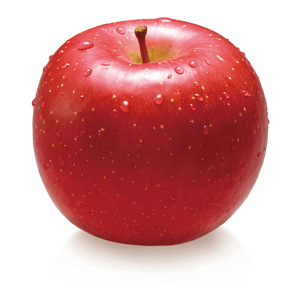
\includegraphics[scale=0.5]{apple02.jpg}
    \caption{りんごの絵}\label{apple-pic-2}
  \end{center}
\end{figure}

国別の詳細を表~\ref{kuni-data}に\newline

図~\ref{apple-pic}はりんごのイメージです

図~\ref{apple-pic-2}はりんごのイメージです


\begin{figure}[ht]
  \begin{center}
    \begin{subfigure}[b]
      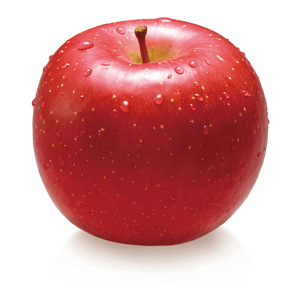
\includegraphics[width=\textwidth]{apple02.jpg}
      \caption{Image 1}
    \end{subfigure} 
    \begin{subfigure}[b]
      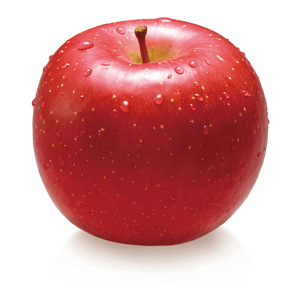
\includegraphics[width=\textwidth]{apple02.jpg}
      \caption{Image 1}
    \end{subfigure} 
    \begin{subfigure}[b]
      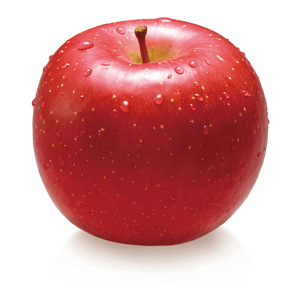
\includegraphics[width=\textwidth]{apple02.jpg}
      \caption{Image 1}
    \end{subfigure} 
    \begin{subfigure}[b]
      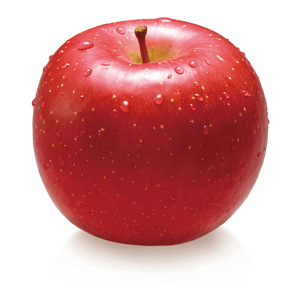
\includegraphics[width=\textwidth]{apple02.jpg}
      \caption{Image 1}
    \end{subfigure} 
    \begin{subfigure}[b]
      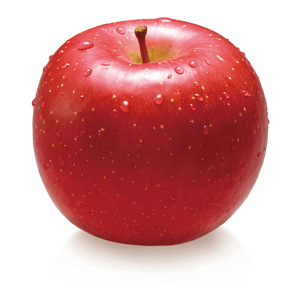
\includegraphics[width=\textwidth]{apple02.jpg}
      \caption{Image 1}
    \end{subfigure} 
  \end{center}
\end{figure}



\end{document}